\documentclass[a4paper,norsk]{article}
\usepackage[utf8]{inputenc}
\usepackage[T1]{fontenc,url}
\usepackage{babel,textcomp}
\usepackage{graphicx, wrapfig}
\usepackage{graphics}
\graphicspath{
	{Code/figs/}
	{Code/scorefigs/}
}
\usepackage{amsmath}
\usepackage{stackengine}
\usepackage{listings}
\usepackage{amsfonts}
\urlstyle {sf}
\title {Project 1 FYS-STK4155 Autumn 2017}
\author {Jon Audun Baar \& Mikael Ravndal}
\begin{document}
\maketitle
All of the plots of the models are done with degree equals 5.
\section*{Introduction}
In this project we were to analyse different sets of data; test-data from the Franke-function and real data, using different linear regression models. The main goal of the project was to evaulate the different models, and come to a conclusion in terms of which models would fit best with which data.
\\Most of our code is in the GitHub repository. We have chosen to not use the code in our report.
\\We have, however, made a python file, project01.py, that provides most of our code in sequence, so that it is possible to follow the code that produce our tests and plots in order.
\section*{Ordinary least square on test data}
First we have generated some test data which we have plotted to get a more intuitive feel for how it looks. We have done this for all the models.
\\Ordinary Least square of the Frankefunction(the same as Ridge with $\lambda=0$):
\\ 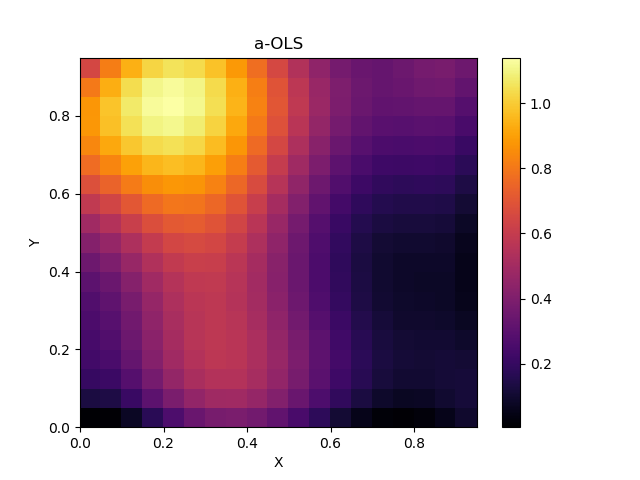
\includegraphics[scale=.7]{a-OLS}
\\As you can tell from our code, we haven't made an own function for ordinary least square, since it is the same as Ridge, just with the $\lambda$ set to 0. This will also show later that when the $\lambda$ gets low it is very similar to OLS.
\\Something something variance etc
\subsection*{Resampling}
Using our bootstrapping algorithm with a resampling of 10, we get these values:
\\
\\VAR: 6.920492.2.
\\BIAS: 945.386100.2.
\\Bootstrap mean of MSE: 0.001121.2.
\\Bootstrap mean of r2Score: 0.985516.2.
\\ 
\\As we can tell
\clearpage
\section*{Ridge regression}
Ridge Regression with $\lambda = 0.1$
\\ 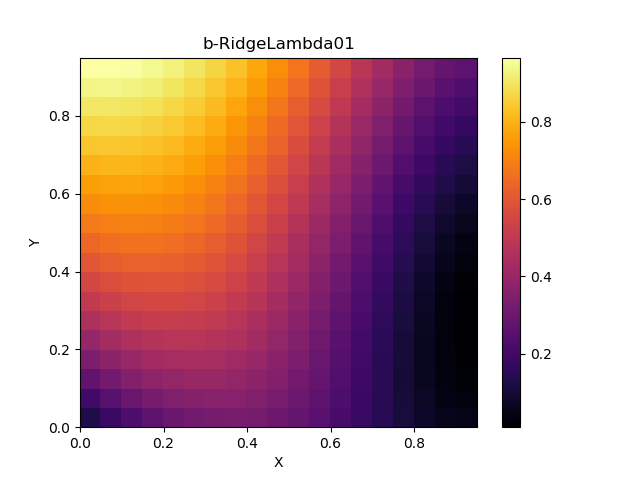
\includegraphics[scale=.7]{b-RidgeLambda01}
\subsection*{Resampling}
We can take a look at how different lambdas and different degrees of the polynomial makes a change in the R2-score and the MSE.
\\Here is a plot to show how they develop as a function of lambda.
\\ 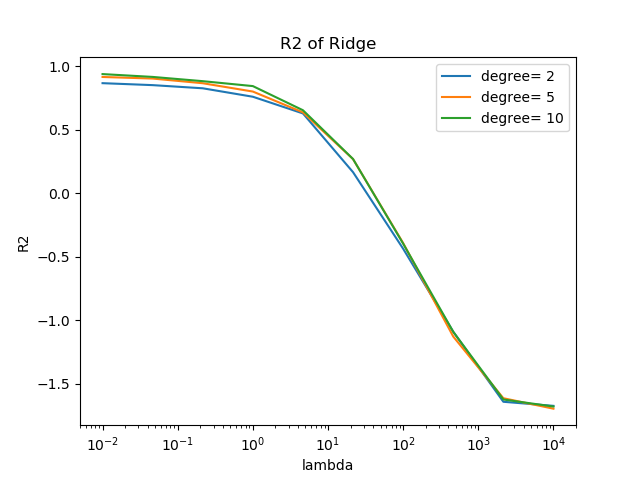
\includegraphics[scale=.7]{MSERidge}
\\ 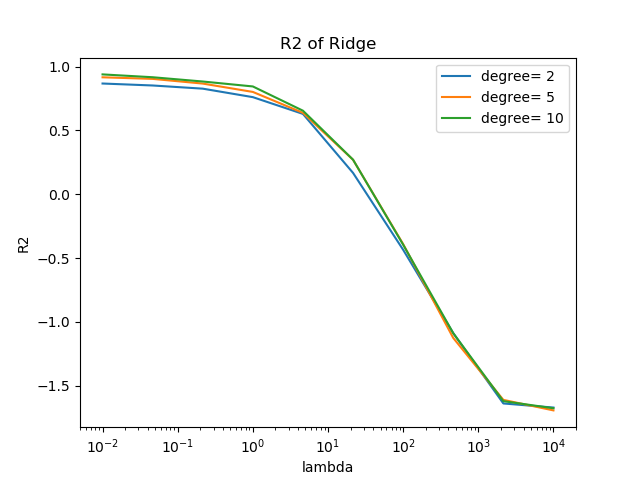
\includegraphics[scale=.7]{R2Ridge}
\\ We can tell pretty easily that the degree of the predictions doesn't matter much, but it varies heavily with lambda.

\clearpage

\section*{Part c)}
Lasso Regression with $\lambda = 0.01$
\\ 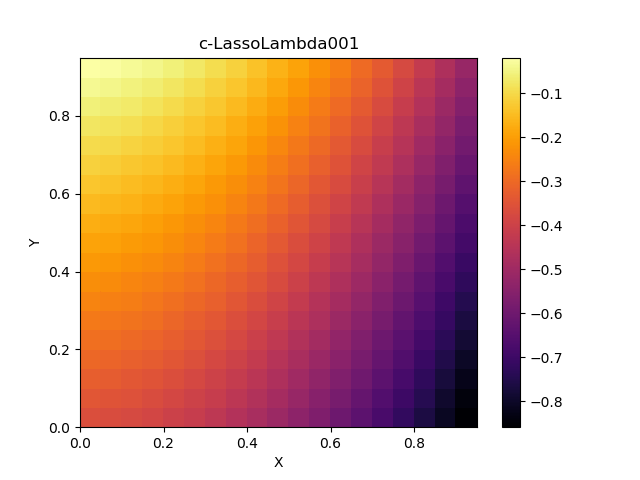
\includegraphics[scale=.7]{c-LassoLambda001}
\clearpage

\section*{Part d)}
Imports 100x100 chunk of real data from top left corner of dataset nr.1.
\\Plot of real data
\\ 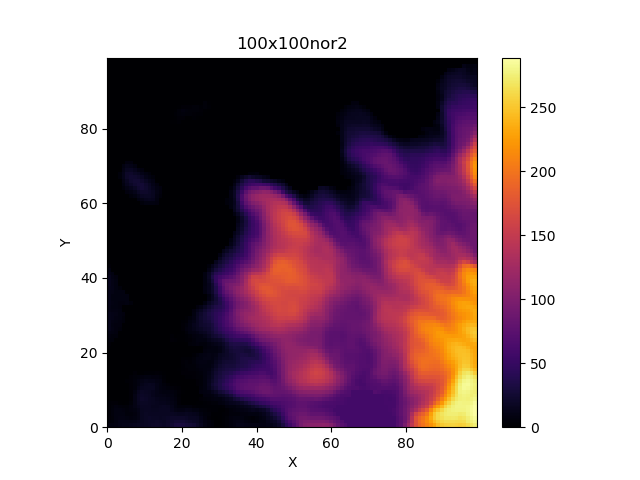
\includegraphics[scale=.7]{100x100nor2}
\clearpage
\section*{Part e)}
Repeat of a-c, but with real data from d)
\\OLS:
\\ 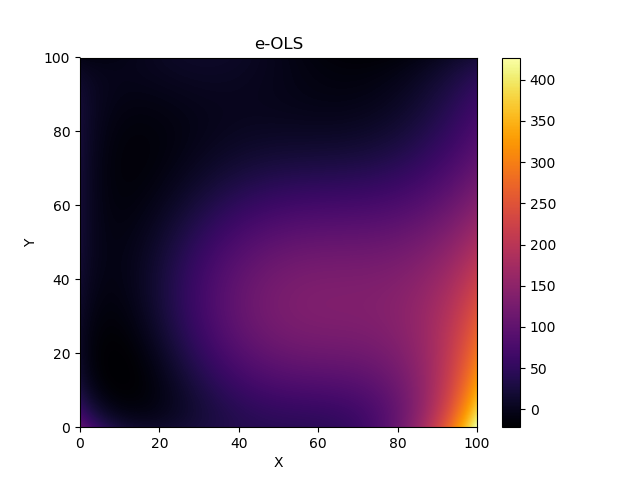
\includegraphics[scale=.7]{e-OLS}
\\Ridge:
\\ 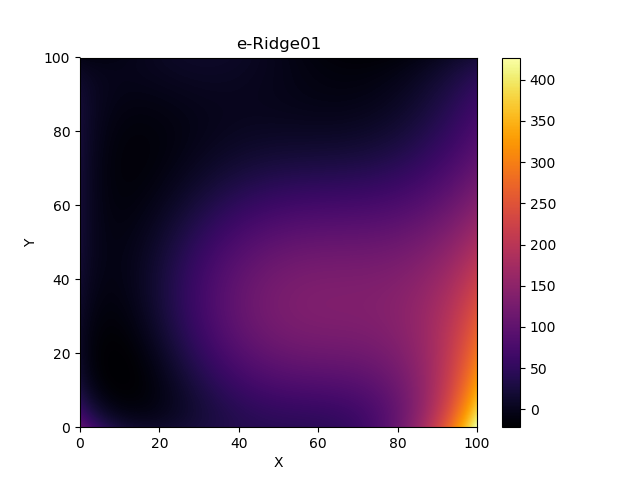
\includegraphics[scale=.7]{e-Ridge01}
\\Lasso:
\\ 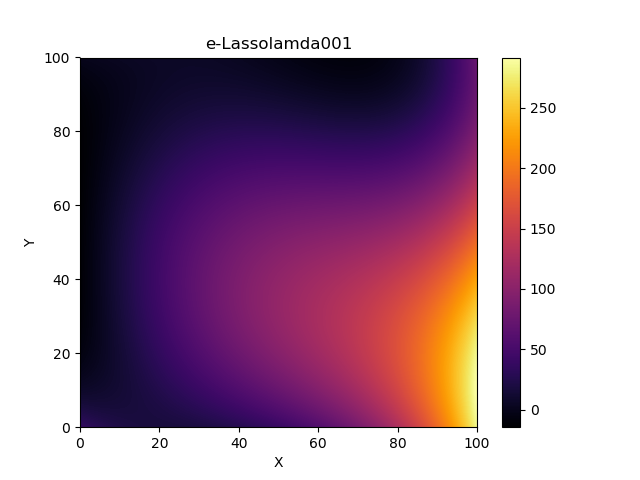
\includegraphics[scale=.7]{e-Lassolamda001}
\end{document}
